\documentclass[10pt,journal,a4paper]{IEEEtran}

\usepackage{color}
\usepackage{overpic}
\usepackage{amssymb}
\usepackage{graphicx}
\usepackage{epstopdf}
\usepackage{amsmath}
\usepackage{graphicx}
\usepackage{amsfonts}
\usepackage{enumitem}
\usepackage{cite}
\usepackage{multirow}
\setlength{\parindent}{0pt}


\title{Appendix}

%\author{Anastasia Tkach\\ 
%Computer Graphics and Geometry Laboratory}

\begin{document}
\maketitle

\section{Convolution segment}

\begin{figure}[h!] 
	\centering
	\hspace{-2em}
	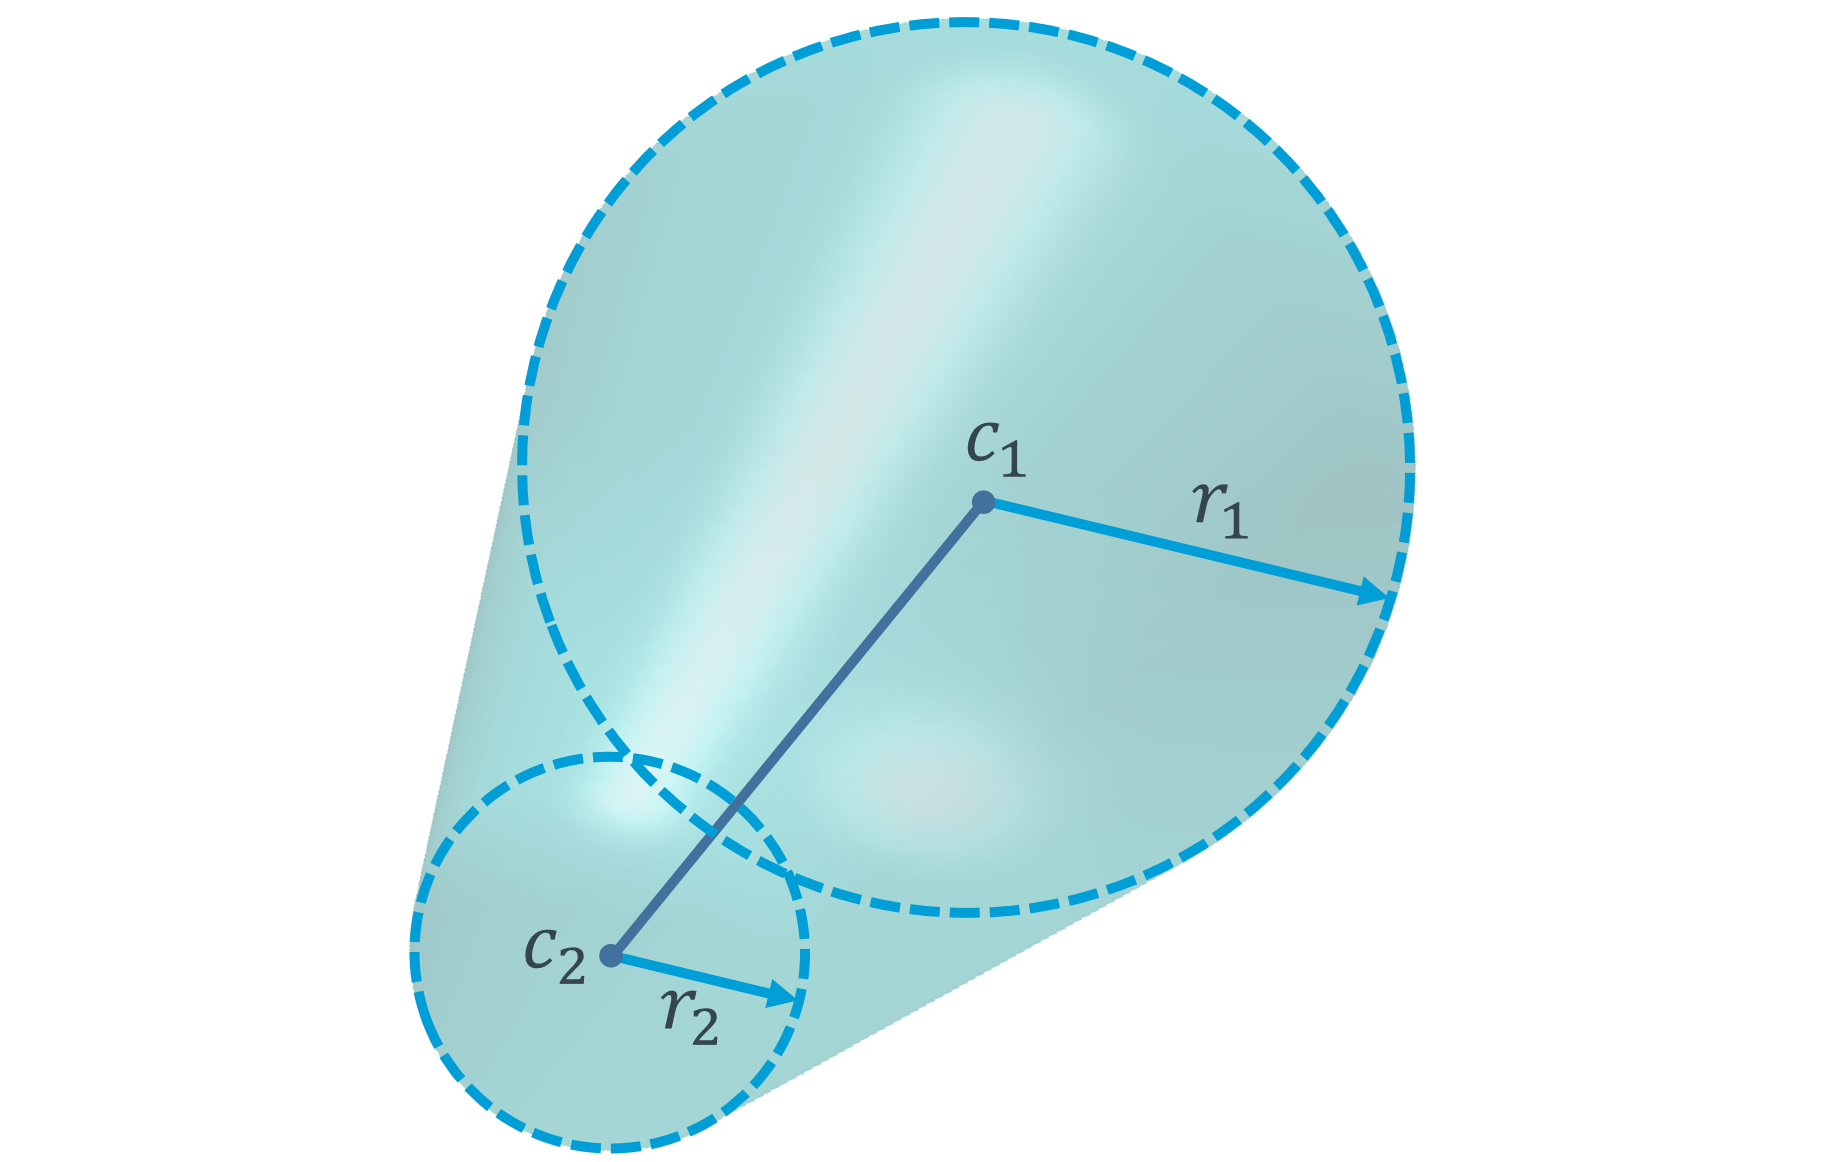
\includegraphics[width=0.3\textwidth]{fig/convsegment.png}
	\caption{Convolution segment.}
	\label{fig:convsegment}
\end{figure}

A convolution segment (Figure \ref{fig:convsegment}) is defined by two spheres $S_1 = \{c_1, r_1\}$ and $S_2 = \{c_2, r_2\}$.
Given the data points $P = \{p_i\}_{i = 1}^N$ and their projections on the model  $Q = \{q_i(c_1, c_2, r_1, r_2)\}_{i = 1}^N$  we construct a vector-function $\textbf{f}$ 

 \begin{equation}
 	\textbf{f} = \left[
 		\begin{array}{c}
 			\vdots \\
			p_i^x - q_i^x\\
			p_i^y - q_i^y\\
			p_i^z - q_i^z\\
			\vdots \\
	\end{array}
 	\right].
 \end{equation} 

\begin{figure}[h!] 
	\centering
	\hspace{-2em}
	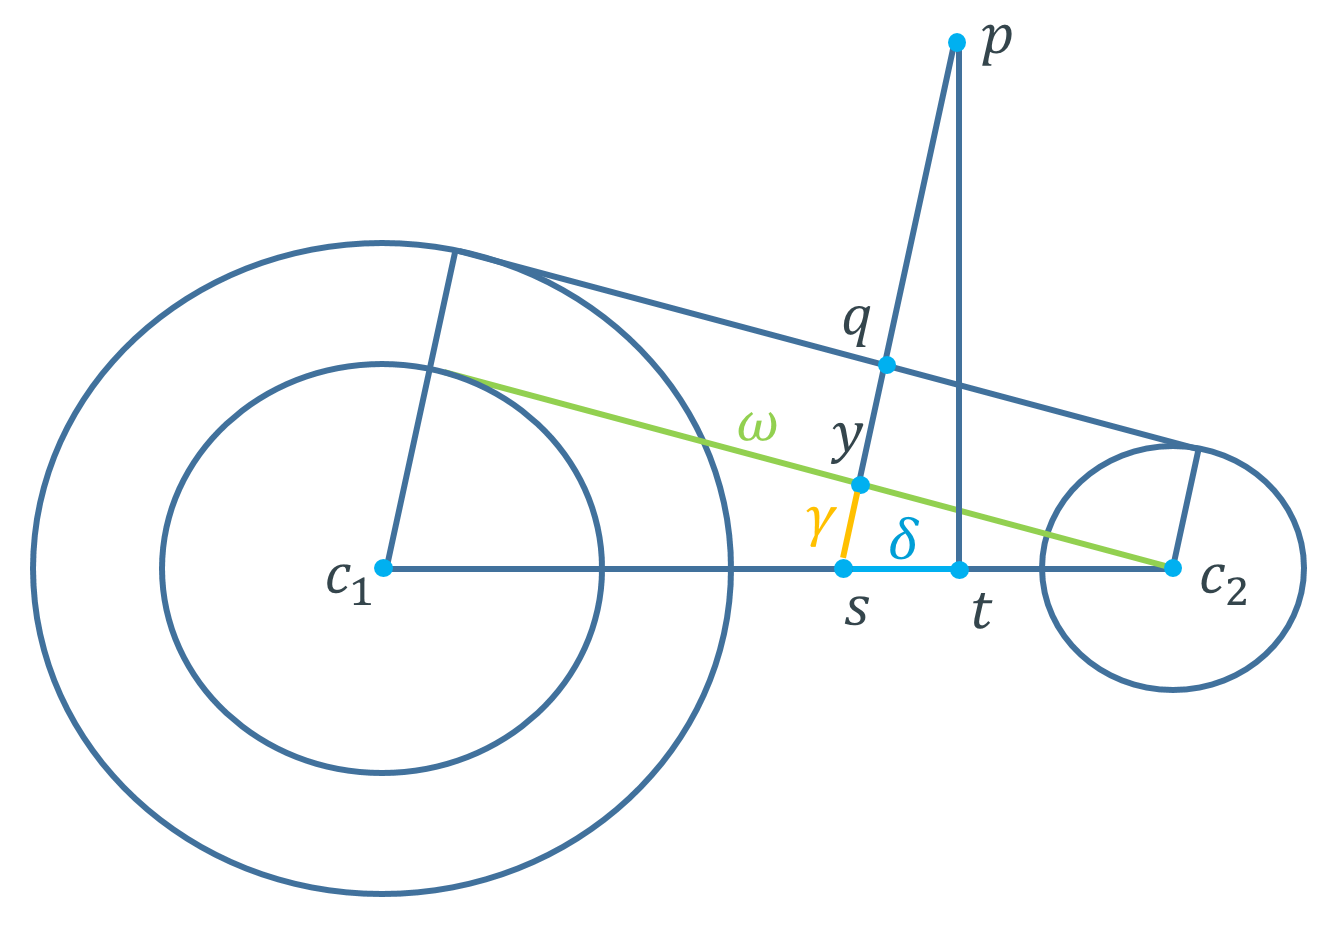
\includegraphics[width=0.47\textwidth]{fig/projection_convsegment.png}
	\caption{Convolution segment.}
	\label{fig:projection_convsegment}
\end{figure}

To fit the model to the data, we iteratively minimize $\textbf{f}$ using Levenberg-Marquardt iteration. In order to compute the Jacobian, the projections $q_i$ should be expressed as functions of model parameters. Let us first find the projection $q$ of a point $p$ on the segment $\{c_1, c_2\}$. Assume that $c_1 > c_2$. If the point on the segment $t$ closest to $p$ lies at the end of the segment, say, $c_1$, than $q = c_1 + \frac{r_1  (p - c_1)}{\Vert p - c_1 \Vert}$. 
Otherwise, the projection $q$ is computed as 

\begin{align*}
& u = c_2 - c_1, \\
& v = p - c_1, \\
& \omega = \sqrt{u^T u - (r_1 - r_2)^2}, \\
&  \delta =  \frac{(r_1 - r_2) \Vert p - t \Vert}{\omega}, \\
&   s = t - \delta  \frac{c_2 - c_1} {\Vert c_2 - c_1 \Vert}, \\
&  \gamma = \frac{(r_1 - r_2)   {\Vert c_2 - t + \delta  \frac{u} {\Vert u \Vert}} \Vert} {\Vert u \Vert}, \\
&   q = s +\frac{ (p - s) (\gamma + r_2) }{ \Vert p - s \Vert } .
\end{align*}

(See Figure \ref{fig:projection_convsegment}).

Given the projection $q_i = q_i(c_1, c_2, r_1, r_2)$, the objective function $\textbf{f} = [\cdots, f_i^T, \cdots]^T$  has the Jacobian $\textbf{J}$ with $J_{ij} = \frac{\partial{f_i}}{\partial{x_j}}$, where $\textbf{x} = [c_1, c_2, r_1, r_2]$.  At each iteration of Levenberg-Marquardt , we first compute the data-model correspondences. In case of convolution segments this amounts to determining whether the closest point is located at one of the end points of the segment or lies in between. Given this correspondence, the Jacobian is computed using chain rule, by composition of derivatives of algebraic operations required to find $q(c_1, c_2, r_1, r_2)$.


%%%%%%%%%%%%%%%%%%%%%%%%%%%%%%%%%%%%%%%%%%%%%%%%%%%%%%%%%%%%%%%%%%%%%%%%


\section{Convolution triangle}


\begin{figure}[h!] 
	\centering
	\hspace{-2em}
	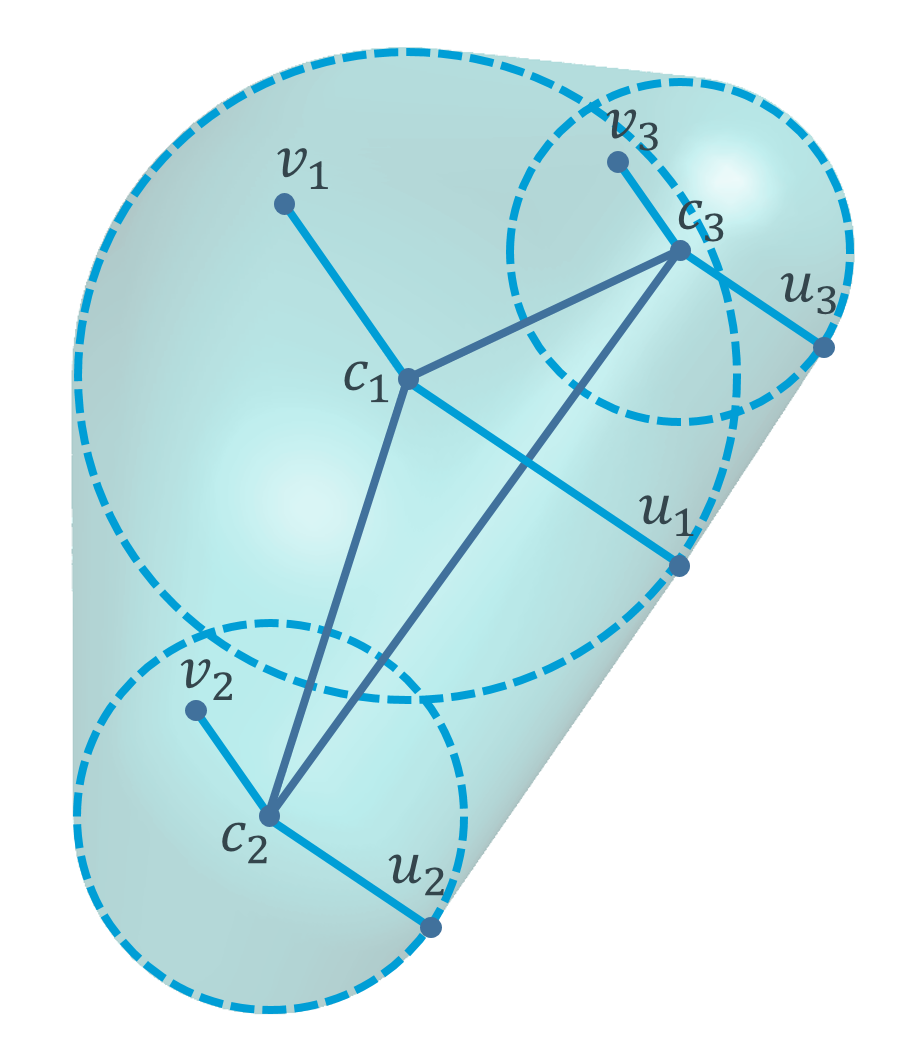
\includegraphics[width=0.3\textwidth]{fig/convtriangle.png}
	\caption{Convolution triangle.}
	\label{fig:convtriangle}
\end{figure}

A convolution triangle (Figure \ref{fig:convtriangle}) is defined by three spheres $S_1 = \{c_1, r_1\}$, $S_2 = \{c_2, r_2\}$ and $S_3 = \{c_3, r_3\}$. To express the projection $q_i$ as a function of the model parameters, first, let us find the outer tangent planes for the spheres. There exists two outer tangent planes if none of the spheres lies entirely inside of the cone tangent to the other two spheres. 

\begin{figure}[h!] 
	\centering
	\hspace{-2em}
	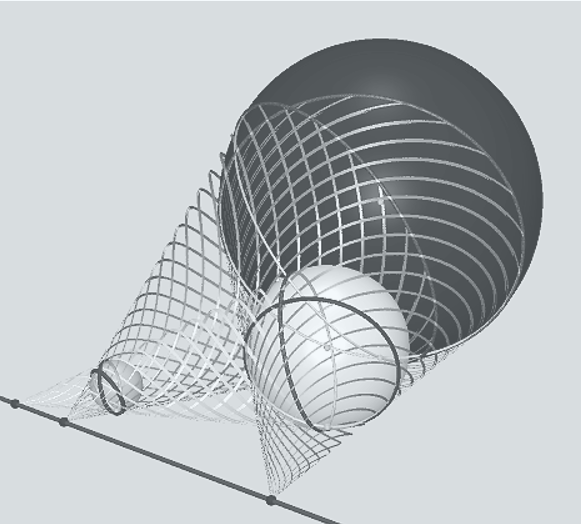
\includegraphics[width=0.45\textwidth]{fig/cones_and_tangent_plane.png}
	\caption{The three apices of the cones tangent to each pair of spheres lie on a straight line.}
	\label{fig:logistic_regression}
\end{figure}

\begin{figure}[h!] 
	\centering
	\hspace{-2em}
	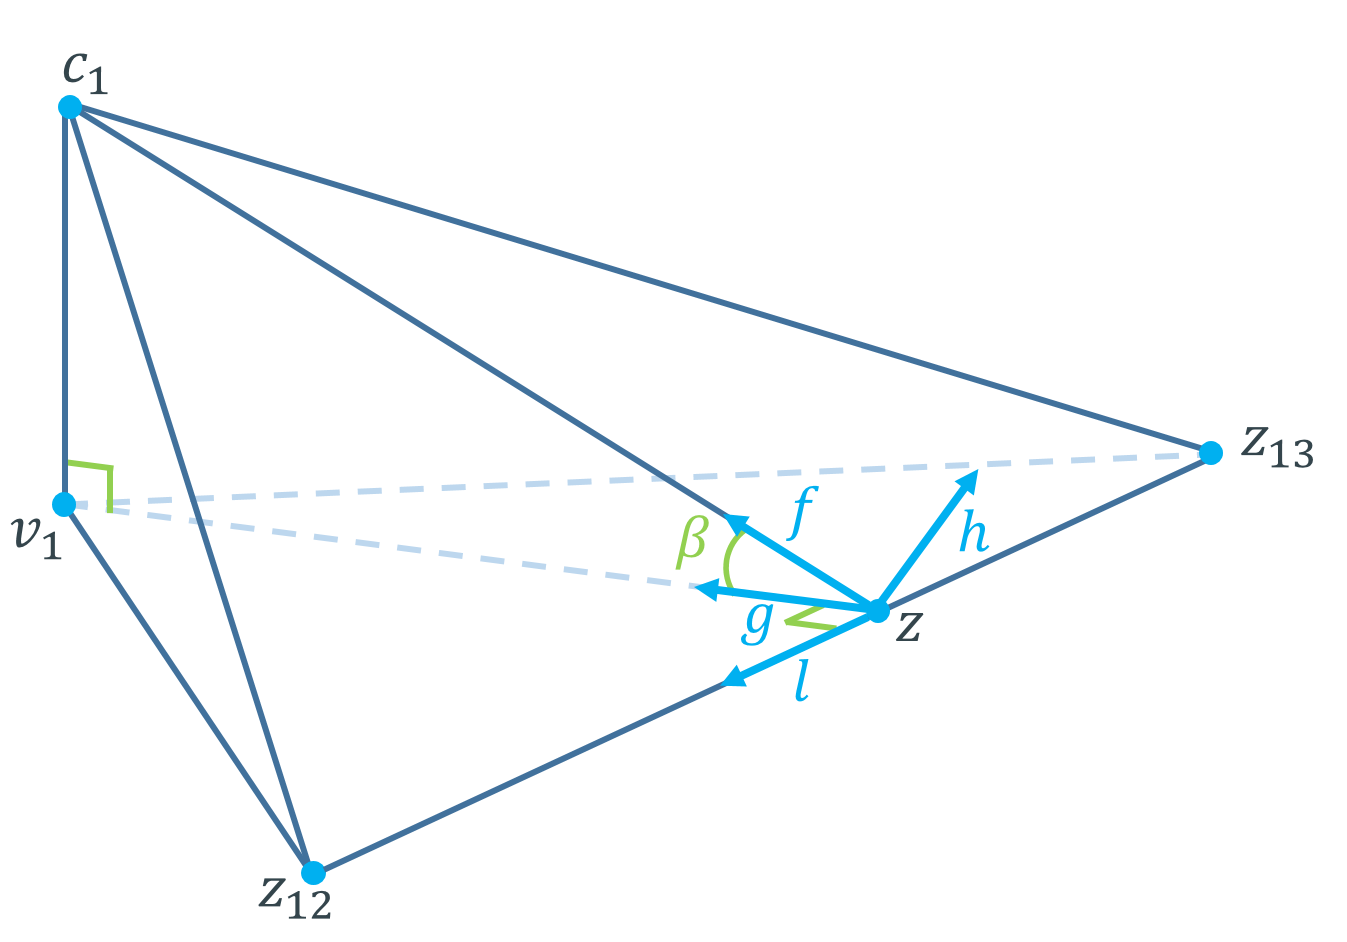
\includegraphics[width=0.45\textwidth]{fig/projection_convtriangle.png}
	\caption{Computing the tangent plane for three spheres.}
	\label{fig:projection_convtriangle}
\end{figure}

\subsection{Computing the tangent plane}

In Figure \ref{fig:projection_convtriangle}, the point $z_{12}$ is an apex of a cone tangent to the spheres $S_1$ and $S_2$. The position of $z_{12}$ can be found from similarity of triangles:

\begin{equation}
	z_{12} = c_1 +\frac{r_1 (c_2 - c_1)}{r_1 - r_2},
\end{equation}

In the same way,

\begin{equation}
	z_{13} = c_1 +\frac{r_1 (c_3 - c_1)}{r_1 - r_3}.
\end{equation}

The direction vector $l$ of the line, that contains the apices of the tangent cones is found as

\begin{equation}
	l = \frac{z_{12} - z_{13}} {\Vert z_{12} - z_{13} \Vert} 
\end{equation}

The intersection point of the plane orthogonal to $l$ and going through the point $c_1$ with the line going through $z_{12}$ and $z_{13}$ is found as

\begin{equation}
z = z_{12} + ((c_1 - z_{12})^T l )l.
\end{equation}

The sine and cosine of the angle $\beta$ in triangle $\{c_1, z, v_1\}$ are given by 

\begin{equation}
	\sin(\beta) = \frac{r_1}{\eta},
\end{equation}

\begin{equation}
	\cos(\beta) = \frac{\nu}{\eta},
\end{equation}

where $\eta = \Vert c_1 - z \Vert $ and $\nu = \sqrt{\eta^2 -  r_1^2}$. 

Denote the tangent point of the sphere $S_1$ as $v_1$. The direction vector $g$ of the line $\{c_1, v_1\}$ can be found by rotating the direction vector $f$ of the line 
$\{c_1, z\}$ by angle $\beta$ around the axis $l$.

\begin{align}
	& h = \frac{l \times f}{\Vert l \times f \Vert}, \\
	& g = \sin(\beta) h + \cos(\beta) f.	
\end{align}

The tangent point $v_1$ is found as
\begin{equation}
v_1 = z + \nu  g
\end{equation}


Having the normal vector of the tangent plane $n = \frac{v_1 - c_1}{\Vert v_1 - c_1 \Vert}$, we can find the tangent points of the spheres $S_2$ and $S_3$:

\begin{align}
	& v_2 = c_2  + r_2 n \\
	& v_3 = c_3 + r_3 n 
\end{align}

The second tangent plane $\{u_1, u_2, u_3$\} is found by rotating the vector $f$ around the axis $l$ by an angle $-\beta$.



\subsection{Computing the projection}

If the point, closest to $p$ on triangle $\{v_1, v_2, v_3\}$ or on triangle $\{u_1, u_2, u_3\}$ lies inside of the triangle, than it is the projection $q$. Otherwise $q$ belongs to the surface of one of the convolution segments $\{c_1, c_2\}$,  $\{c_1, c_3\}$, or  $\{c_1, c_3\}$. Thus, the candidates for $q$ are the projections of $p$ on the segments $q_{12}$, $q_{13}$ or $q_{23}$. The projection $q$ is determined taking into account the distance to $p$ and whether  $q_{12}$, $q_{13}$ and $q_{23}$ are located inside or outside of the segments $\{c_1, c_2\}$,  $\{c_1, c_3\}$, and  $\{c_1, c_3\}$.  

%%%%%%%%%%%%%%%%%%%%%%%%%%%%%%%%%%%%%%%%%%%%%%%%%%%%%%%%%%%%%%%%%%%%%%%%

\section{Combining several blocks}

Consider the case when several convolution segments and triangles are used to create a more complex model. To find the projection $q$, we compute a projection $q_j$ on each  building block.  The projection $q$ is determined taking into account the distances between $q_j$ and $p$ and whether  $q_j$ are located inside or outside of the building blocks.

%%%%%%%%%%%%%%%%%%%%%%%%%%%%%%%%%%%%%%%%%%%%%%%%%%%%%%%%%%%%%%%%%%%%%%%%


%\bibliographystyle{plain}
%\bibliography{htrack}

\end{document}
